\documentclass[10pt,a4paper]{article}

\usepackage{gensymb}
\usepackage{hyperref}

% COMMON PACKAGES

% ---------------------------------------------------------------------------
% --- Mateatyka
% ---------------------------------------------------------------------------
\usepackage{amsmath,bm,amsfonts,amssymb}    % wzory, równania, symbole matematyczne
\usepackage{wasysym}                        % inne symbole i znaki matematuczne (np. promil)
\RequirePackage{siunitx}    				% SI unit HTU \si{}

% ---------------------------------------------------------------------------
% --- Jezyki
% ---------------------------------------------------------------------------
\usepackage[T1]{fontenc}
\usepackage[utf8]{inputenc}     % okresla system kodowania tekstu
\usepackage[polish]{babel}

% ---------------------------------------------------------------------------
% --- Marginesy
% ---------------------------------------------------------------------------
\usepackage[top=2.5cm, bottom=2.5cm, left=2.5cm, right=2.5cm]{geometry} % ustawienia marginesów
\RequirePackage{kantlipsum} % English kantian-style lipsum (wypełniacze tekstu)
\RequirePackage{lipsum}     % Lorem ipsum (wypełniacze tekstu)

% ---------------------------------------------------------------------------
% --- Kolory i makra
% ---------------------------------------------------------------------------
\usepackage{xcolor}                         % definiowanie kolorów
\newcommand{\myRed}[1]{\textcolor{red}{#1}} % wykorzystanie makro \myRed{tekst}
\definecolor{GIKorange}{HTML}{C06000}       % definiowanie własnego koloru
\newcommand{\myOrange}[1]{\textcolor{GIKorange}{#1}} % wykorzystanie makro \myOrange{tekst}

\definecolor{pw_sloneczny}{RGB}{254, 213, 66}
\definecolor{pw_morelowy}{RGB}{234, 124, 90}
\definecolor{pw_mietowy}{RGB}{106, 186, 156}
\definecolor{pw_sliwkowy}{RGB}{150, 95, 119}
\definecolor{pw_szafirowy}{RGB}{120, 150, 207}
\definecolor{pw_wrzosowy}{RGB}{180, 160, 170}
\definecolor{pw_grafitowy}{RGB}{60, 60, 76}
\definecolor{pw_mokka}{RGB}{100, 90, 90}

% ------------------------------------------------------------------------------------------------------------
% --- Wstawianie rysunków
% ------------------------------------------------------------------------------------------------------------
\usepackage{graphicx}       % wstawianie grafiki
\DeclareGraphicsExtensions{.pdf,.eps,.png,.jpg}

\usepackage{float}          % to fix table/figure location \begin{figure}[ht]
\usepackage{subfloat}       % subfigure options
\usepackage{caption}            
\usepackage{subcaption}


\usepackage{array}
\usepackage{multicol}       % \multicolumn{num_cols}{alignment}{contents}
\usepackage{multirow}       % \multirow{''num_rows''}{''width''}{''contents''} {* for the width means the content's natural width}
\usepackage{longtable}  % Multi-page tables
\usepackage{booktabs}       % tabele (toprule/midrule/bottomrule)
\usepackage{tabularx}   % to wrap words (here use in enviroment condition)
%--------------------------------
% CONDITIONS: A new enviroments  to explain parameters in equations
%--------------------------------
\newenvironment{conditions*}
{\par\vspace{\abovedisplayskip}\noindent
	\tabularx{\columnwidth}{>{$}l<{$} @{${}: {}$} >{\raggedright\arraybackslash}X}}
{\endtabularx\par\vspace{\belowdisplayskip}}

% ------------------------------------------------------------------------------------------------------------
% --- Wstawianie hyperlinków i ulr
% ------------------------------------------------------------------------------------------------------------
\usepackage[obeyspaces,spaces]{url}     % wstawianie ścieżek i stron www np.:  \path{/home/kinga/doc/file}  or \url{www.....}
\usepackage{hyperref}                   % wstawianie odniesień (hyperlinks)
% ----- HYPEREF SETUP 
\hypersetup{hidelinks,
	bookmarks=true,
	bookmarksopen=true,
	colorlinks=true,            % hyperlinks will be coloured
	linkcolor=pw_mietowy,            % hyperlink text will be green
	linkbordercolor=black,      % hyperlink border will be red
	citebordercolor=black,      % color of links to bibliography
	citecolor=black,
	filebordercolor=black,      % color of file links
	urlbordercolor=black,       % color of external links
	filecolor=black,
	menucolor=black,
	urlcolor=black,
	backref= page,              % page, section(s)
	pagebackref = true,         % to show number of page with citations backref=none
	plainpages=true,            % false
	pdfpagelabels,
	hypertexnames=true,         % false
	linktocpage}


% ----- modyfikacja pakietu hyperref aby jedynie podkreślał link
%\makeatletter
%\Hy@AtBeginDocument{%
%\def\@pdfborder{0 0 1}% Overrides border definition set with colorlinks=true
%\def\@pdfborderstyle{/S/U/W 1}% Overrides border style set with colorlinks=true
%                              % Hyperlink border style will be underline of width 1pt
%}
%\makeatother

%--------------------------------------
% Bibiography specification ver PL
%--------------------------------------
\RequirePackage[natbibapa]{apacite}	    % bibliography natbib - natbibapa loads the natbib package for the citation commands
\bibliographystyle{apacite}
%\nocite{*} % uzyj aby uwzględnić wszystkie odniesienia w bazie danych .bib (bez tego jedynie cytowane pozycje)
\renewcommand{\BBAA}{i}  % between authors in parenthetical cites and ref. list
\renewcommand{\BBAB}{i}  % between authors in in-text citation
\renewcommand{\BAnd}{i}  % for ``Ed. \& Trans.'' in ref. list
\renewcommand{\BOthers}{i in}
\renewcommand{\doiprefix}{DOI:}
\urlstyle{APACrm}



% ------------------------------------------------------------------------------------------------------------
% --- Wstawianie fragmentów kodu
% ------------------------------------------------------------------------------------------------------------
%--------------------------------------
% Code  listings and verbatim ()
%--------------------------------------
\usepackage{courier}               % to keep bold for \ttfamily
\usepackage{verbatim}              % environment which looks for the exact string 
\usepackage{pmboxdraw}             % alows to use special unicode character U + 20000
\RequirePackage{listings}              % Code listings
\RequirePackage{ucs}                   % tosupportencodingutf8x.
\renewcommand{\lstlistingname}{Kod}    % put the name of caption 
% general option of listing
\lstset{aboveskip       = 1.mm,
	belowskip       = 1.mm,
	frame           = single,
	numbers         = left,
	firstnumber     = 1,
	xleftmargin     = 2em,
	numberstyle     = {\footnotesize},
	basicstyle      ={\footnotesize\ttfamily}, % \ttfamily
	breaklines      = true,
	backgroundcolor = \color{pw_grafitowy!1!white},
	commentstyle    = \color{pw_grafitowy!85!white}\textit,
	stringstyle     = \color{pw_grafitowy},
	keywordstyle    = \bfseries,
	otherkeywords   = {def, return, assert, with, try, exept, Lambda, Map, Fiter, yield, nonlocal, bytes, Ellipsis, NotImplemented, None, setdefault, read, readline, readlines, write, writeline, close, self, SyntaxError, ZeroDivisionError, SyntaxError, IndentationError, IndexError, AssertionError, KeyError, TypeError, NameError, AttributeError, ValueError, RuntimeError,False, True},                
	breaklines      = true,
	postbreak=\mbox{\textcolor{red}{\rotatebox[origin=c]{180}{$\Lsh$}}\space}, % break line for long text
	inputencoding   = utf8x, % incorporate polish characters
	extendedchars   = \true,
	literate={ą}{{\k{a}}}1
	{Ą}{{\k{A}}}1
	{ę}{{\k{e}}}1
	{Ę}{{\k{E}}}1
	{ó}{{\'o}}1
	{Ó}{{\'O}}1
	{ś}{{\'s}}1
	{Ś}{{\'S}}1
	{ł}{{\l{}}}1
	{Ł}{{\L{}}}1
	{ż}{{\.z}}1
	{Ż}{{\.Z}}1
	{ź}{{\'z}}1
	{Ź}{{\'Z}}1
	{ć}{{\'c}}1
	{Ć}{{\'C}}1
	{ń}{{\'n}}1
	{Ń}{{\'N}}1
}


   % ścieżka względna do katalogu z ustawieniami
\graphicspath{{images/}}    % stała ścieżka względna do katalogu z  obrazkami.

\newcommand{\logoGIK}{settings/WGiK-znak.png}
\newcommand{\authorName}{Agata Wyrzykowska  \\ grupa 3, Numer Indeksu: 312109}

\newcommand{\titeReport}{Projekt 1, 12.04.2022r.}
\newcommand{\titleLecture}{Informatyka geodezyjna \\ sem. IV, projekt, rok akad. 2021-2022}
\newcommand{\kind}{report}
\newcommand{\mymail}{\href{mailto:01160139@pw.edu.pl}{01160139@pw.edu.pl}}
\newcommand{\supervisor}{....}
\newcommand{\gikweb}{\href{www.gik.pw.edu.pl}{www.gik.pw.edu.pl}}
\newcommand{\institut}{Zakład Geodezji Wyższej i Astronomii}
\newcommand{\faculty}{Wydział Geodezji i Kartografii}
\newcommand{\university}{Politechnika Warszawska}
\newcommand{\city}{Warszawa}
\newcommand{\thisyear}{2022}

\pdfinfo
{
	/Title       (GIK PW)
	/Creator     (TeX)
	/Author      (Agata Wyrzykowska)
}

% ------------------------- POCZATEK DOKUMENTU -------------------
\begin{document}
	% ----------------------------------------------------------------
	% ----------------------------  Title page
	% ----------------------------------------------------------------
	\begin{center} 
		\rule{\textwidth}{.5pt} \\
		\vspace{1.0cm} %odstep pionowy
		\includegraphics[width=.4\paperwidth]{\logoGIK}
		\vspace{0.5cm} \\
		\Large \textsc{\titeReport}
		\vspace{0.5cm} \\  
		\large \textsc{\titleLecture}
		\vspace{0.5cm}\\
		\textsc{\authorName}  \\
		\mymail \\
		\textsc{\faculty}, \textsc{\university}  \\ 
		\city, \today
	\end{center} 
	\rule{\textwidth}{1.5pt}
	
	
	% ---------------------------------------------------------------
	% ----------------------------  Table of content
	% ----------------------------------------------------------------
	\tableofcontents 								% wyświetla spis treści
	%\addcontentsline{to}{chapter}{Spis treści} 	% dodaje pozycję do spisu treści
	% \listoffigures  								% wyświetla spis rysunków
	%\addcontentsline{toc}{chapter}{Lista rysunków} % dodaje pozycję do spisu treści
	% \listoftables 									% wyświetla spis rysunków
	%\addcontentsline{toc}{chapter}{lista tabel}	% dodaje pozycję do spisu treści
	\newpage
	
	\section{Opis zadania}
	
	W celu wykonania pierwszego projektu należało przygotować aplikację która będzie potrafiła przeliczać dowolne współrzędne. Aby sprawdzić poprawność napisanego programu należało również wykonać napisać kod testujący wszystkie napisane w nim funkcje. Dodatkowo został napisany również pseudokod oraz schemat blokowy podanych w programie funkcji. \\
	Wszystkie pliki z programami oraz plik ze współrzędnymi należało zaimportować do GitHuba: \href{https://github.com/jkluvm/projek1informatyka}{\textbf{link do strony internetowej z kodem programu}}.
	
	\subsection{Instrukcja obsługi programu.}
	Całość aplikacji została napisana w klasie. Na samym początku należy skorzystać z funkcji inicjującej, która pozwoli nam zdefiniować rodzaj elipsoidy i na podstawie wybranych parametrów będzie można opierać swoje dalsze obliczenia. Do wyboru można mamy elipsoidę \textbf{GRS80} oraz \textbf{WGS84}. W przypadku wybrania innej dowolnej elipsoidy program zwróci informację, że dana elipsoida nie została zaimportowana do funkcji i należy skorzystać z którejś z powyższych. Po wyznaczeniu dużej i małej półosi, algorytm oblicza również spłaszczenie Ziemi oraz kwadrat mimośrodu.\\
	\\
	Następną funkcją w programie jest funkcja \textbf{dms}, która służy do zamiany stopni dziesiętnych na stopnie, minuty i sekundy z dokładnością do pięciu miejsc po przecinku. Nie jest ona niezbędna, służy tylko i wyłącznie stylistycznemu  przedstawieniu wyników w stopniach. \\
	\\
	Następną funkcją jest \textbf{hirvonen}, który jest algorytmem transformującym współrzędne ortokartezjańskie na geodezyjne z dokładnością do ok. 1 cm. Do jej uruchomienia algorytmu należy podać współrzędne X, Y, Z dowolnego punktu. Funkcja korzysta również z parametrów elipsoidy wyznaczanych przez funkcję inicjującą. \\
	\\
	Kolejna funkcja jest odwrotną do hirvonena - \textbf{blh2xyz}. Służy do przekształcania współrzędnych geodezyjnych na ortokartezjańskie. Wykorzystuje parametry elipsoidy wyznaczone w funkcji inicjującej. \\
	\\
	Funkcja \textbf{xyz2neu} służy do przekształcania współrzędnych ortokartezjańskich na topocentryczne. Aby ją zainicjować należy podać współrzędne dwóch dowolnych punktów. Wykorzystany jest w nim opisany wyżej algorytm hirvonena, który pozwoli nam wyznaczyć fi, lam, h wybranego z punktów, które sa konieczne do wyznaczenia macierzy. \\
	\\
	Następnym algorytmem jest funkcja \textbf{uklad1992}, która zamienia przestrzenne współrzędne geodezyjne fi, lam na współrzędne płaskie x, y. W tej części również są wykorzystywane parametry elipsoidy z funkcji inicjującej. \\
	\\
	Na tej samej zasadzie działa funkcja \textbf{uklad2000}, jest ona jednak nieco bardziej skomplikowana, gdyż posiada wiele warunków, w zależności od tego w której części kraju znajdą się odwzorowywane punkty geodezyjne. \\
	\\
	Ostatnią funkcją jest algorytm \textbf{katy odl}, który wyznacza kąt azymutu i elewacji oraz odległości 2D i 3D między punktami. Aby wywołać funkcję, należy podać współrzędne ortokartezjańskie dwóch dowolnych punktów na powierzchni Ziemi. \\
	\newpage
	
	\section{Schematy blokowe wybranych funkcji}
	\subsection{Funkcja inicjująca parametry elipsoidy}
	\begin{center}
		\newcommand{\model}{settings/model.png}
		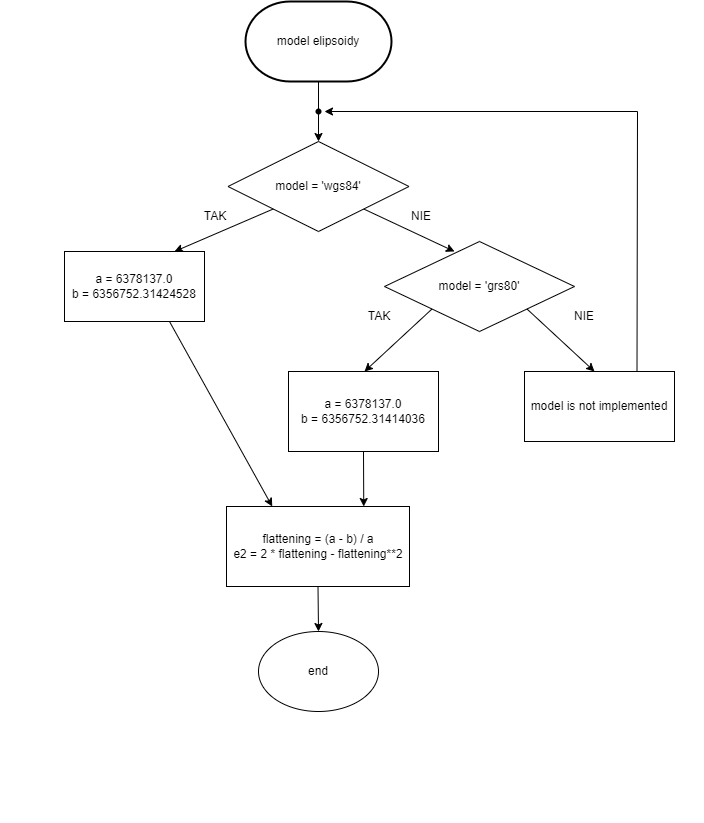
\includegraphics[width=.8\paperwidth]{\model}
	\end{center}
	\newpage
	
	\subsection{Funkcja hirvonen}
	\begin{center}
		\newcommand{\hirvonen}{settings/hirvonen.png}
		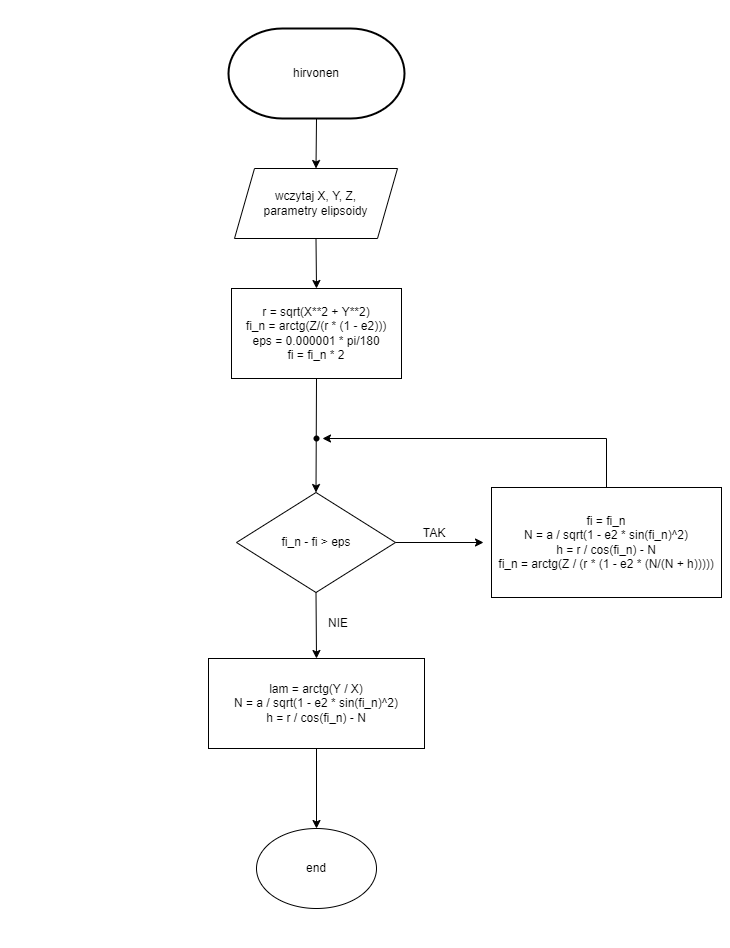
\includegraphics[width=.8\paperwidth]{\hirvonen}
	\end{center}
	\newpage
	
	\subsection{Funkcja blh2xyz}
	\begin{center}
		\newcommand{\blhxyz}{settings/blh2xyz.png}
		\includegraphics[width=.8\paperwidth]{\blhxyz}
	\end{center}
	\newpage
	
	\subsection{Funkcja xyz2neu}
	\begin{center}
		\newcommand{\xyzneu}{settings/xyz2neu.png}
		\includegraphics[width=.8\paperwidth]{\xyzneu}
	\end{center}
	
	\subsection{Funkcja uklad1992}
	\begin{center}
		\newcommand{\uklad}{settings/uklad1992.png}
		\includegraphics[width=.7\paperwidth]{\uklad}
	\end{center}

	\subsection{Funkcja uklad2000}
	\begin{center}
		\newcommand{\ukladd}{settings/uklad2000.png}
		\includegraphics[width=.6\paperwidth]{\ukladd}
	\end{center}
	
	\subsection{Funkcja katy odl}
	\begin{center}
		\newcommand{\katy}{settings/katy.png}
		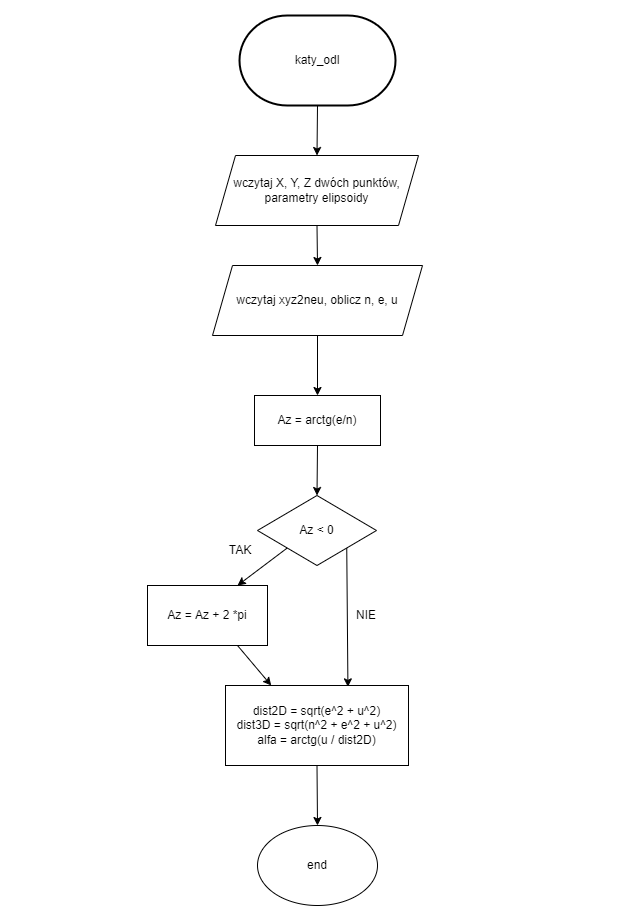
\includegraphics[width=.7\paperwidth]{\katy}
	\end{center}
	
	\newpage
	\section{Pseudokod}
	\rule{\textwidth}{.5pt} \\
	Wybierz jedną z funkcji: \\
	1. \textbf{init}: \\
	wyznacz model elipsoidy na bazie której będą wykonywane transformacje \\
	2. \textbf{dms} \\
	przekształć kąty dziesiętne na kąty wyrażone w stopniach, minutach i sekundach do pięciu miejsc po przecinku \\
	3. \textbf{hirvonen} \\
	wykonaj transformację ze współrzędnych geocentrycznych na geodezyjne \\
	4. \textbf{blh2xyz} \\
	wykonaj transformacje ze współrzędnych geodezyjnych na geocentryczne \\
	5. \textbf{xyz2neu} \\
	wykonaj transformacje ze współrzędnych geocentrycznych na współrzędne topograficzne \\
	6. \textbf{uklad1992} \\
	wykonaj transformacje ze współrzędnych geodezyjnych na współrzędne płaskie układu 1992 \\
	7. \textbf{uklad2000} \\
	wykonaj tranformacje ze współrzędnych geodezyjnych na współrzędne plaskie układu 2000 \\
	8. \textbf{katy odl} \\
	wykonaj algorytm na wyznaczenie kąta azymutu, kąta elewacji oraz odległości 2D i 3D \\
	\rule{\textwidth}{.5pt} \\
	
\end{document}